\section{Experiments and Results}
\label{ch4:sec:final_exp_res}
We investigate the effectiveness of the proposed models on 2D airfoil optimization cases following the settings in ADODG Case 1. The optimization objective is to reduce the drag coefficient of NACA-0012 in a transonic inviscid flow (Ma=0.85) at zero angle-of-attack. To demonstrate the benefits of the proposed model's full differentiability, we use different methods to evaluate the airfoil's drag coefficient and generate the CFD's gradients (i.e. surface sensitivities or uncertainties) with respect to the geometry. Specifically, we use a GCNN \cite{aa.Baque2018} surrogate model and SU2's adjoint solver \cite{aa.Economon2016}, respectively.
In the remainder of this paper, we use terms like \textit{LSM + SU2} to represent a pair of parameterization model and evaluation model.

\subsection{The Evaluation Modules}
\subsubsection{The GCNN Surrogate Model}
The GCNN takes the airfoil's connected contour as input and extracts geometric features based on the vertices and edges. It predicts the drag coefficient in two ways. ${C_d}^{int}$ is obtained by predicting air pressure values per vertex and computing an integral of pressure over the airfoil's surface and ${C_d}^{direct}$ is obtained by predicting an overall drag coefficient directly. The minimization objective is a summation of both predictions as $C_d = {C_d}^{int} + {C_d}^{direct}$.

The GCNN network structure consists of 5 graph convolution blocks, each with 3 convolutional layers. Batch normalization \cite{ai.Ioffe2015} is used after each layer and the Exponential Linear Unit \cite{ai.Clevert2015} is used as an activation function. The model is trained using the Adam optimizer with a learning rate of $5 \times 10^{-4}$ for 900 epochs.

\subsubsection{The SU2 Adjoint Solver}
We use SU2's continuous adjoint solver to calculate the sensitivity scale of the drag minimization objective along the surface's vertex normal direction using the simulation result. To avoid the non-uniqueness issue of the Euler equation \cite{aa.Masters2017,aa.LeDoux2015}, we employ a restart strategy for flow field initialization \cite{aa.He2019}. During optimization, we gradually change the airfoil's geometry between successive iterations with a moderate learning rate for the parameterization model to ensure the optimization result converges to a satisfying minimum. We speedup this process by updating the adjoint result at regular intervals and reusing the SU2 gradient for multiple iterations, given that adjoint solving takes considerably more time than evaluating a surrogate model. In case of numerical instability, we discard the SU2's gradient if its norm becomes excessively large, even if the minimum residual criteria are met.

\subsection{The Geometric Constraints}
The overall geometric constraint can be generically expressed as a weighted sum of $P$ task specific constraints, $Q$ parameterization model specific constraints and $R$ evaluation model specific constraints: $\cL_{cons} = \sum_{i=1}^P w_{T,i}C_{T,i} + \sum_{j=1}^Q w_{M,j}C_{M,j} + \sum_{k=1}^R w_{E,k}C_{E,k}$, where $C_T$ is defined by the optimization objective, $C_M$ is defined by the parameterization models and $C_E$ is defined by the evaluation modules. $w_{T,i}$, $w_{M,j}$ and $w_{E,k}$ are weights for the corresponding constraints.

\subsubsection{Task Specific Constraints}
We denote the geometric constraint of ADODG Case 1 as the bounding constraint $C_{T,1}$, which limits the airfoil’s thickness from decreasing below its initial value and writes
\begin{equation}
    {C_{T,1}} = \frac{1}{{|{V^S}|}}\sum\limits_{i = 1}^{|{V^S}|} \left|\left|{\max (|{v}_{y,i}^{S,opt}| - |{v}_{y,i}^{S,init}|,0)}\right|\right|^2\;\;,
\end{equation}
where ${v}_{y,i}^{S,opt}$ and ${v}_{y,i}^{S,init}$ are $y$ coordinates of surface vertices from the optimized airfoil and the initial airfoil, respectively.

\begin{figure}[!tb]
    \begin{center}
        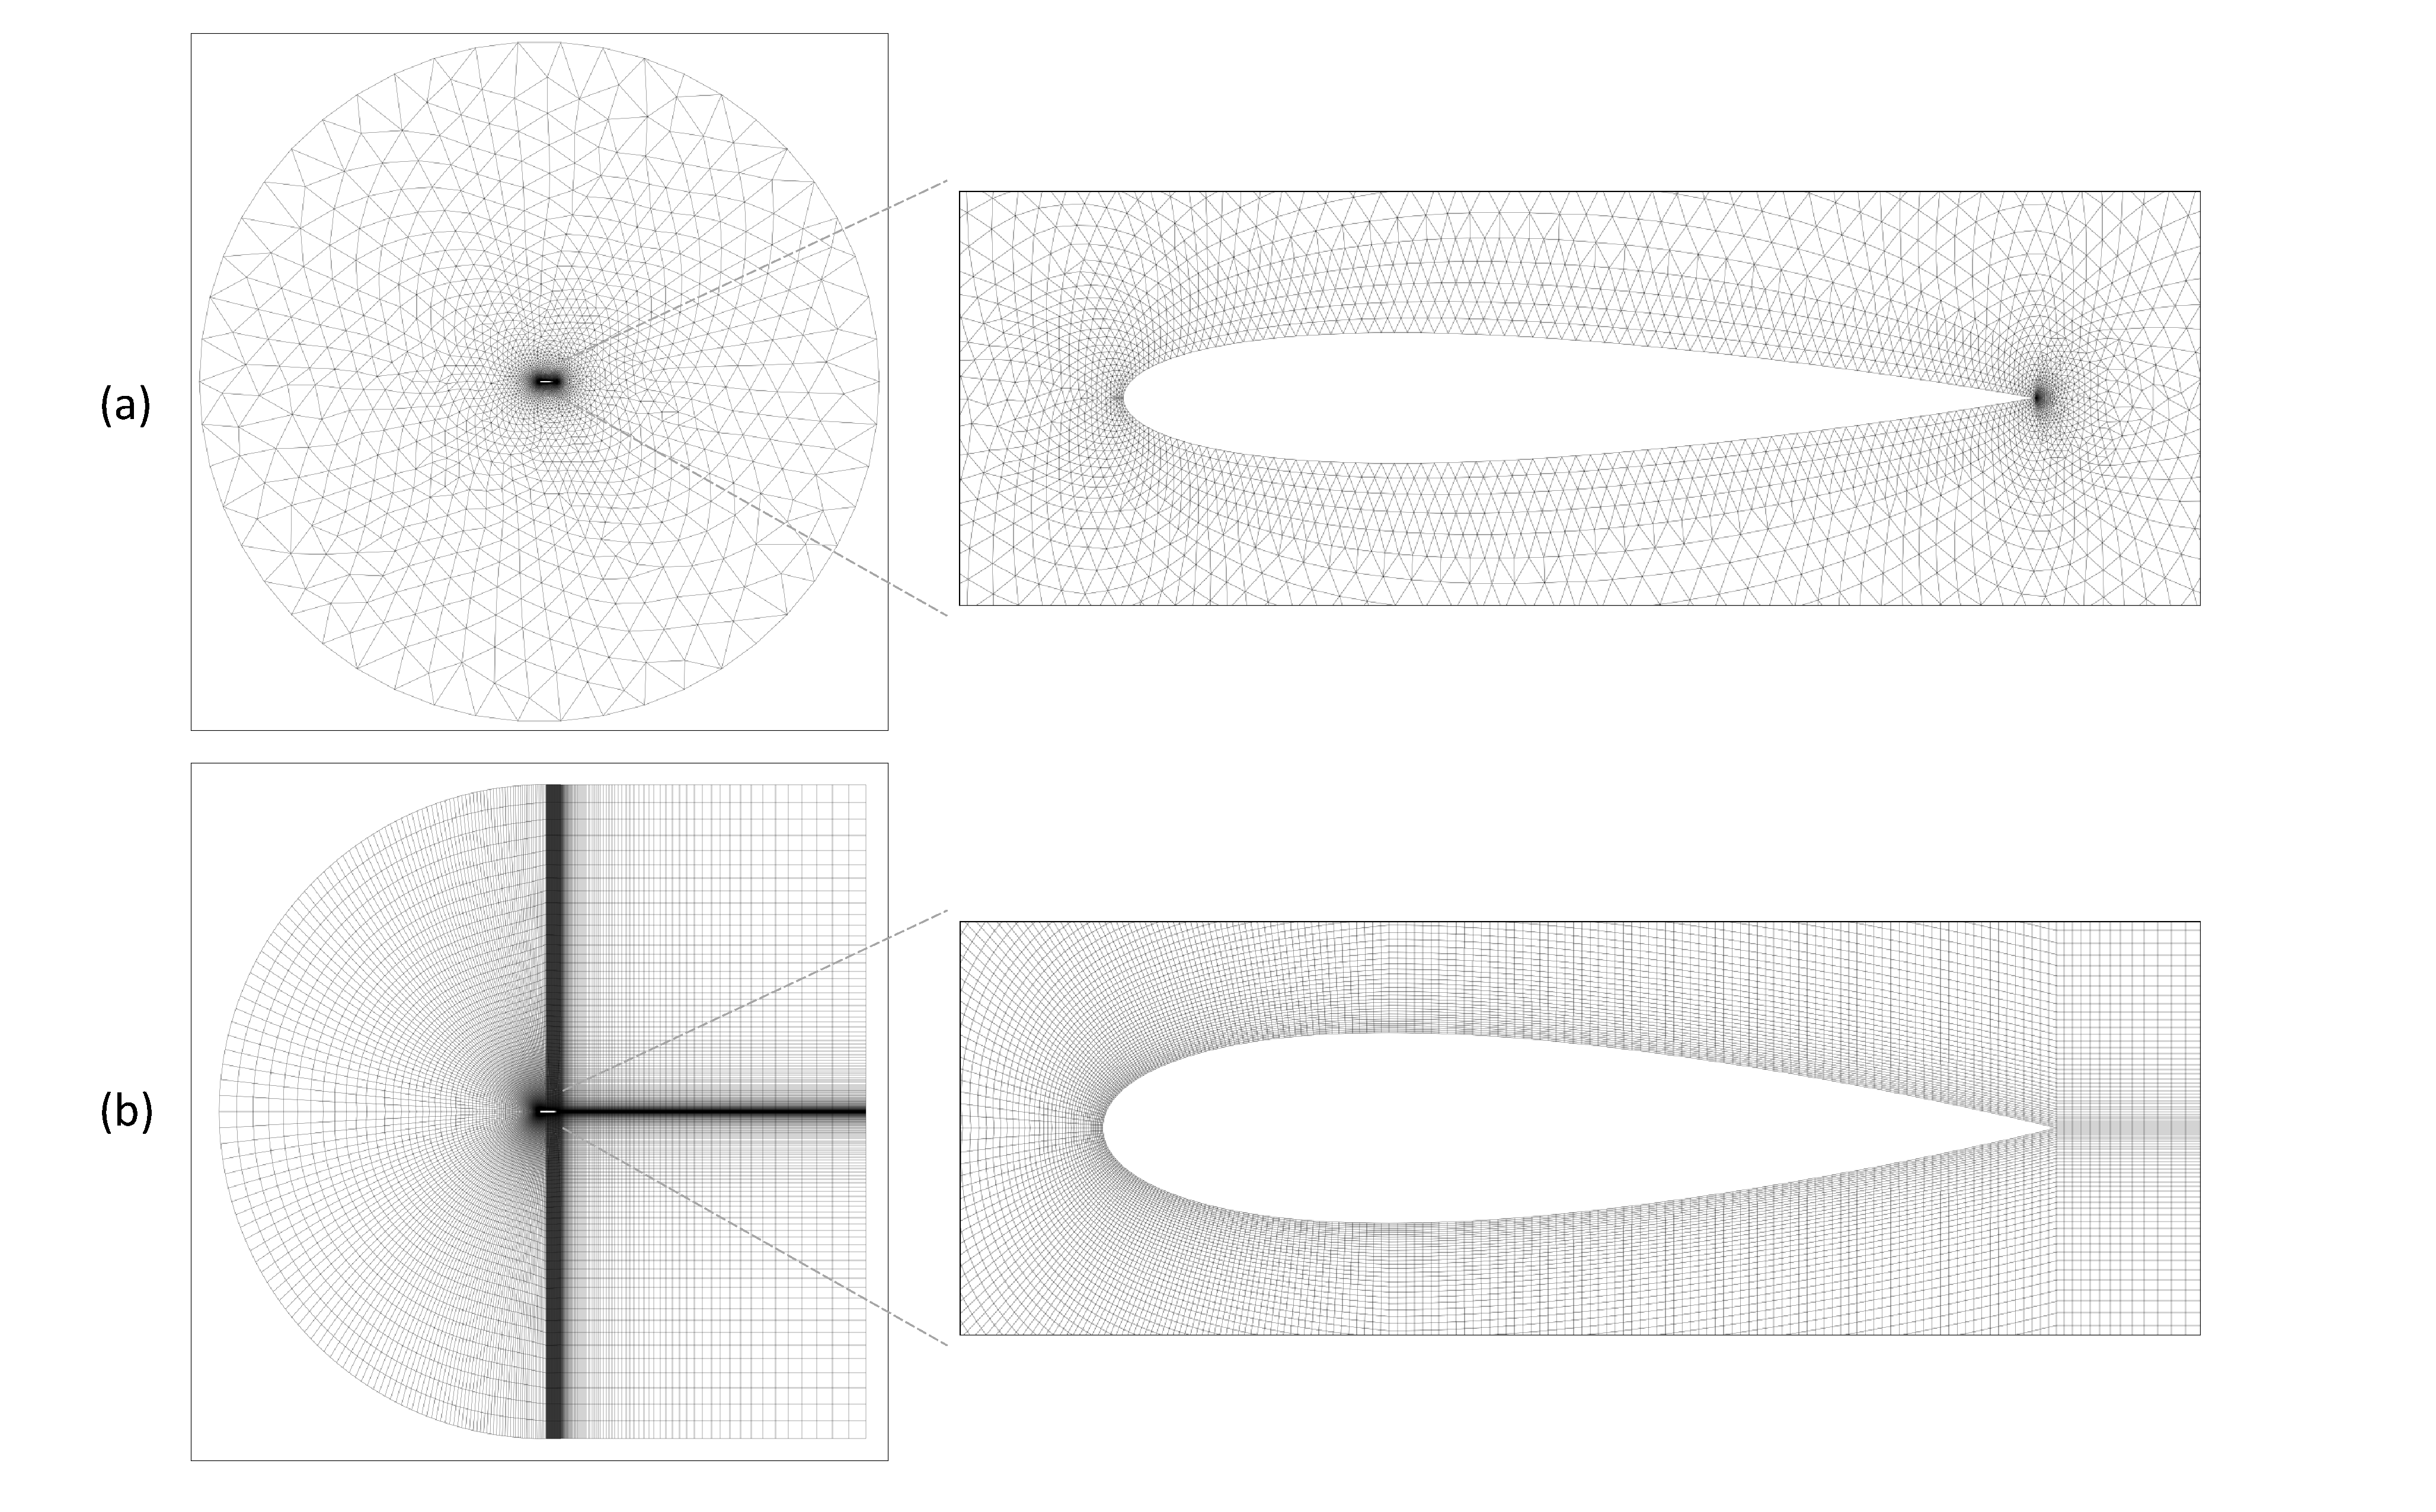
\includegraphics[width=0.9\linewidth]{chapter4/fig/template_meshes.pdf}
    \end{center}
    \caption{
        \small The two template meshes employed in the adjoint solver based shape optimization experiments: (a) \textit{TM-A} and (b) \textit{TM-B}. Both meshes are built on NACA-0012.
    }
    \label{ch4:fig:template_meshes}
\end{figure}


\subsubsection{Parameterization Model Specific Constraints}
For LSM, we define a constraint on the norm of latent code $\bz$, i.e. $C_{M,1}$, to ensure that the optimized $\bz^*$ falls within the latent distribution learned from the training data, and the generated airfoil is valid, which writes
\begin{equation}
    C_{M,1} = ||\bz||^2_F\;\;.
\end{equation}

For DMM, we fix the leading edge $\bv_{leanding}^S$ and trailing edge $\bv_{trailing}^S$ and constrain the $x$ coordinate to maintain the normalized chord length and chord position. We denote these constraints as $C_{M,2}$ and $C_{M,3}$, respectively, which write
\begin{equation}
    C_{M,2}=\left|\left| \bv_{leanding}^S - [0,0] \right|\right|^2 + \left|\left| \bv_{trailing}^S - [1,0] \right|\right|^2\;\;,
\end{equation}
\begin{equation}
    C_{M,3}=\sum_i^{|V^S|} \left|\left| \max (0 - \bv_{x,i}^S, 0) + \max (\bv_{x,i}^S - 1, 0) \right|\right|^2\;\;.
\end{equation}

\subsubsection{Evaluation Module Specific Constraints}
Since SU2 calculates the sensitivity scale along the surface normal direction, applying this gradient to the mesh model will result in a redistribution of surface vertices, leading to subsequent non-orthogonality in the volumetric cells directly connected to them. To address this issue, we define a constraint $C_{E,1}$ that decays the horizontal shifting as
\begin{equation}
    C_{E,1} = \sum_i^{|V^S|} \left|\left| \delta\bv_{x,i}^S
 \right|\right|^2\;\;.
\end{equation}
The GCNN does not require any additional constraints.

\subsubsection{Constraints on Computational Mesh}
When both models are combined with an adjoint solver, we again use the regularization loss as a constraint on the quality of the computational mesh, specifically $C_{M,4}=\cL_{reg}$. 

In summary, \textit{LSM + GCNN} uses $\{C_{T,1},C_{M,1}\}$, \textit{LSM + SU2} uses $\{C_{T,1},C_{M,1},C_{E,1}\}$, \textit{DMM + GCNN} uses $\{C_{T,1},C_{M,2},C_{M,3}\}$ and \textit{DMM + SU2} uses $\{C_{T,1},C_{M,2},C_{M,3},C_{E,1}\}$.

\begin{table}[tbp]
  \centering
  \caption{Quantitative comparison with previous shape optimization methods with handcrafted and semi-automatic parameterizaations on ADODG Case I benchmark. The drag coefficients are reported in counts. (1 count = $10^{-4}$)}
    \begin{tabular}{l|c|c}
    \hline
    Models & Initial $C_d$ & Optimized $C_d$ \\
    \hline
    He et al. \cite{aa.He2019} & 470.36  & 7.60  \\
    He et al. \cite{aa.He2019} & 470.36  & 15.54  \\
    He et al. \cite{aa.He2019} & 470.36  & 23.53  \\
    Masters et al. \cite{aa.Masters2016} & 469.60  & 25.00  \\
    Bisson and Nadarajah \cite{aa.Bisson2015} & 464.20  & 26.20  \\
    He et al. \cite{aa.He2019} & 470.36  & 34.33  \\
    Carrier et al. \cite{aa.Carrier2014} & 471.20  & 36.70  \\
    Lee et al. \cite{aa.Lee2015} & 457.33  & 42.24  \\
    He et al. \cite{aa.He2019} & 470.36  & 50.49  \\
    \textit{DMM + SU2} & 466.11  & 69.32  \\
    Zhang et al. \cite{aa.Zhang2016} & 481.28  & 73.08  \\
    Poole et al. \cite{aa.Poole2015b} & 469.42  & 83.80  \\
    LeDoux et al. \cite{aa.LeDoux2015} & 471.30  & 84.50  \\
    Gariepy et al. \cite{aa.Gariepy2015} & 481.60  & 141.70  \\
    \textit{DMM + GCNN} & 466.11  & 278.23  \\
    \textit{LSM + SU2} & 466.11  & 283.93  \\
    Fabiano and Mavriplis \cite{aa.Fabiano2016} & 466.96  & 297.02  \\
    \textit{LSM + GCNN} & 466.11  & 354.91\\
    \hline
    \end{tabular}%
  \label{ch4:tab:result}%
\end{table}%
\begin{figure}[!htb]
    \begin{center}
        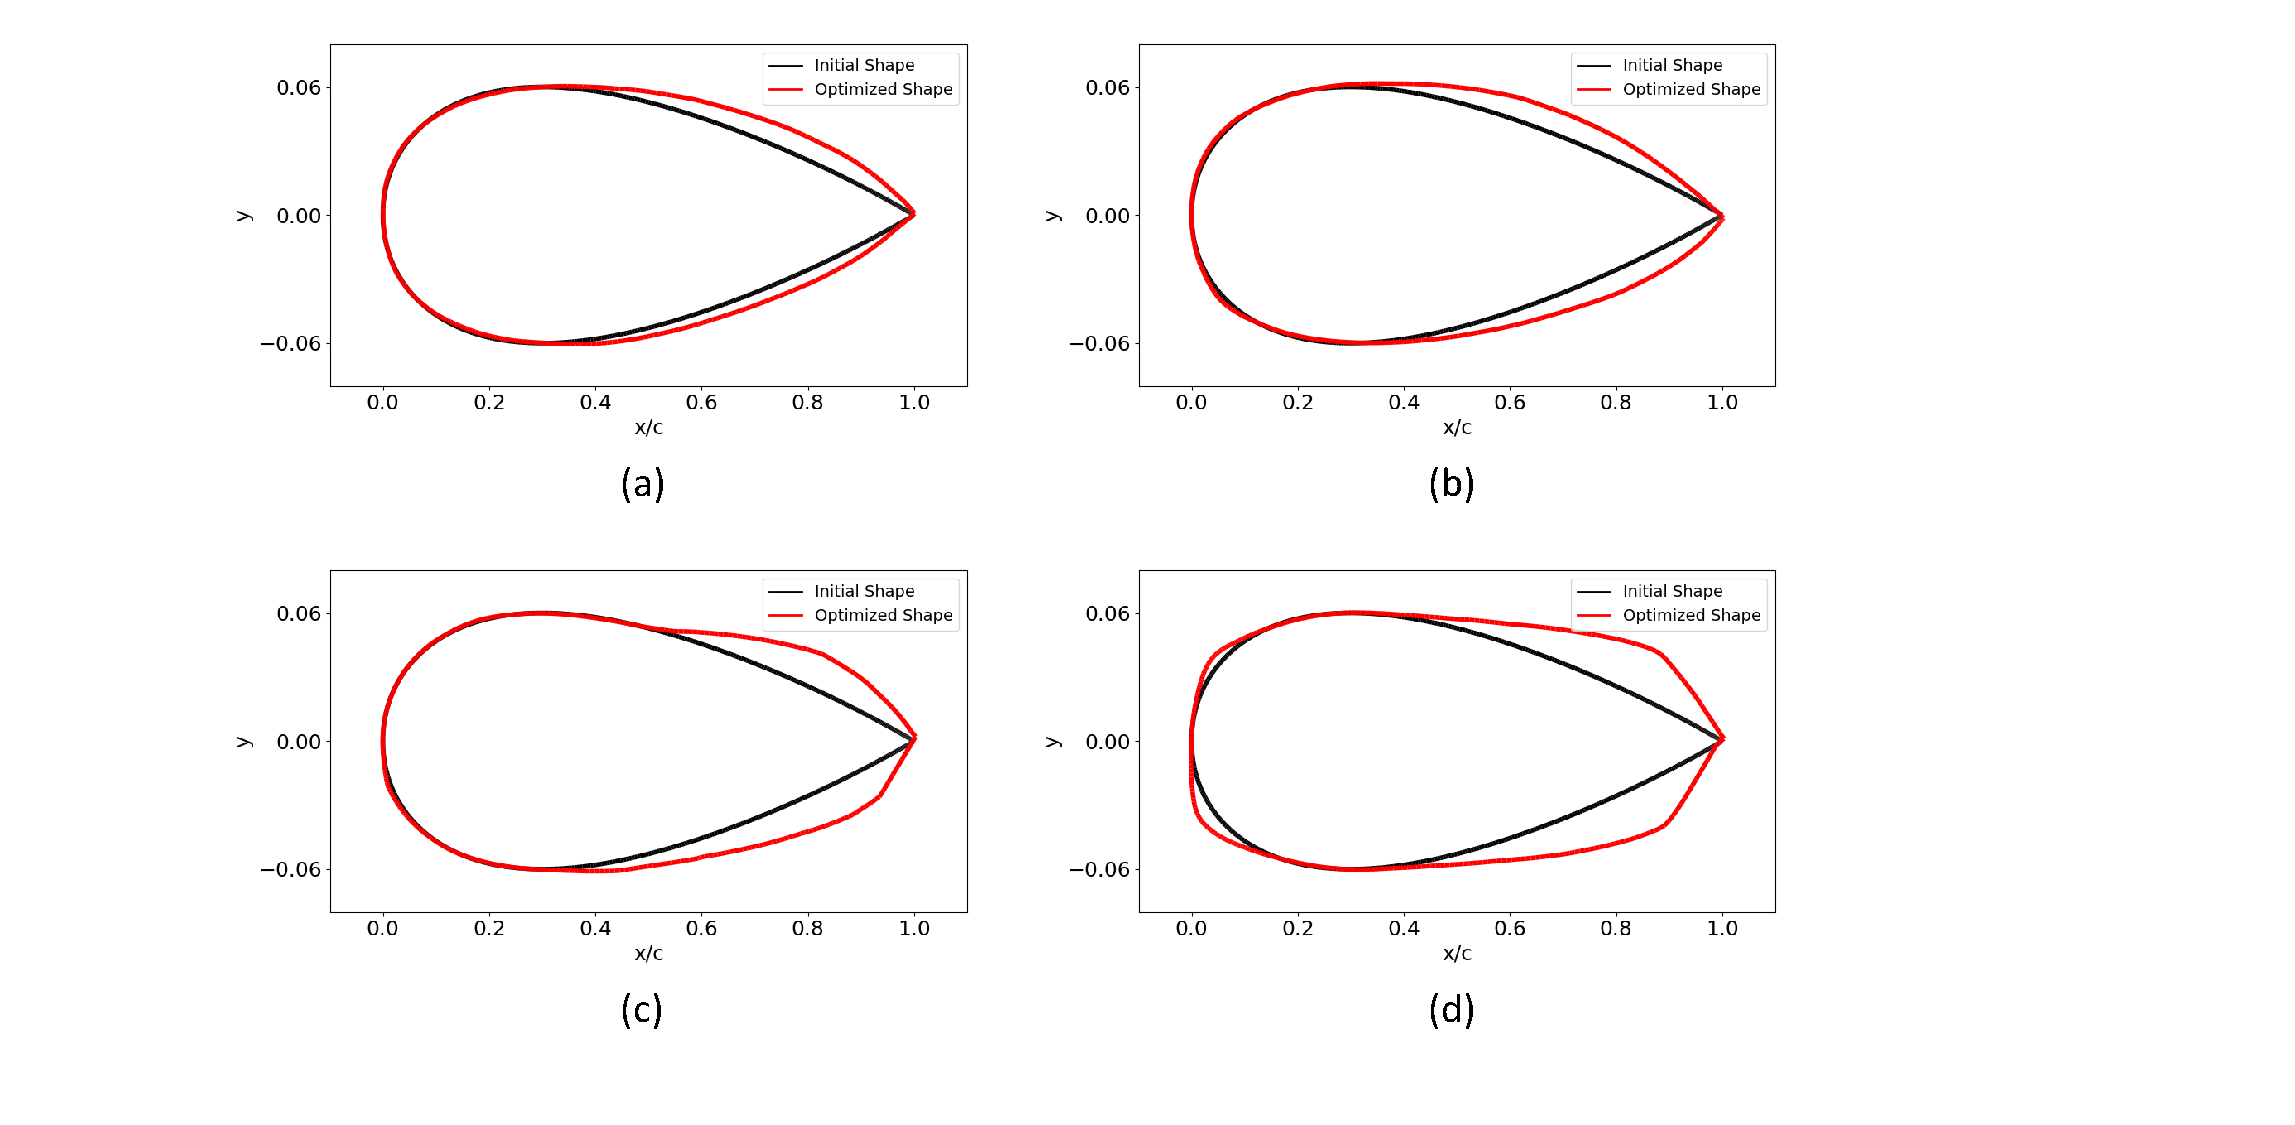
\includegraphics[width=1\linewidth]{chapter4/fig/final_optim_result.pdf}
    \end{center}
    \caption{
        \small The shape optimization results of (a) \textit{LSM + GCNN}, (b) \textit{LSM + SU2}, (c) \textit{DMM + GCNN} and (d) \textit{DMM + SU2}. The initial NACA-0012 and optimized shapes are colored in black and red.
    }
    \label{ch4:fig:final_optim_results}
\end{figure}

\subsection{Shape Optimization Results}
When using SU2 for optimization, we accelerate the process by using the coarse template mesh \textit{TM-A}~\footnote{\url{https://github.com/su2code/Tutorials/blob/master/design/Inviscid_2D_Unconstrained_NACA0012/mesh_NACA0012_inv.su2}} for most iterations. Once the drag coefficient stops reducing, we switch to a fine template mesh \textit{TM-B}~\footnote{\url{http://www.wolfdynamics.com/tutorials.html?id=148}} for the final iterations. Fig.\ref{ch4:fig:template_meshes} illustrates these template meshes. \textit{TM-A} consists of $5233$ vertices and $10126$ triangles, while \textit{TM-B} consists of $58120$ vertices and $57600$ quadrilateral cells.
When using GCNN for optimization, the choice of template mesh is not important, as GCNN only requires the airfoil's contour as input.

Meanwhile, we introduce a reparameterization mechanism to prevent catastrophic mesh errors terminating the iterations during optimization. When $C_{M,4}$ becomes large or both simulation and adjoint solving fail to meet the residual criteria, we sample points $S'$ from the current airfoil surface $f_{\Theta}(\bz,\hat{\bv}^S)$ or $g_{\Phi}(\hat{\bv}^S)$ and update $\bz$ for LSM or $\Phi$ for DMM using Eq. \ref{ch4:eq:agmin_f_z} or Eq. \ref{ch4:eq:agmin_g_phi}. Then the optimization continues on the reparameterized model.

\begin{figure}[!htb]
    \begin{center}
        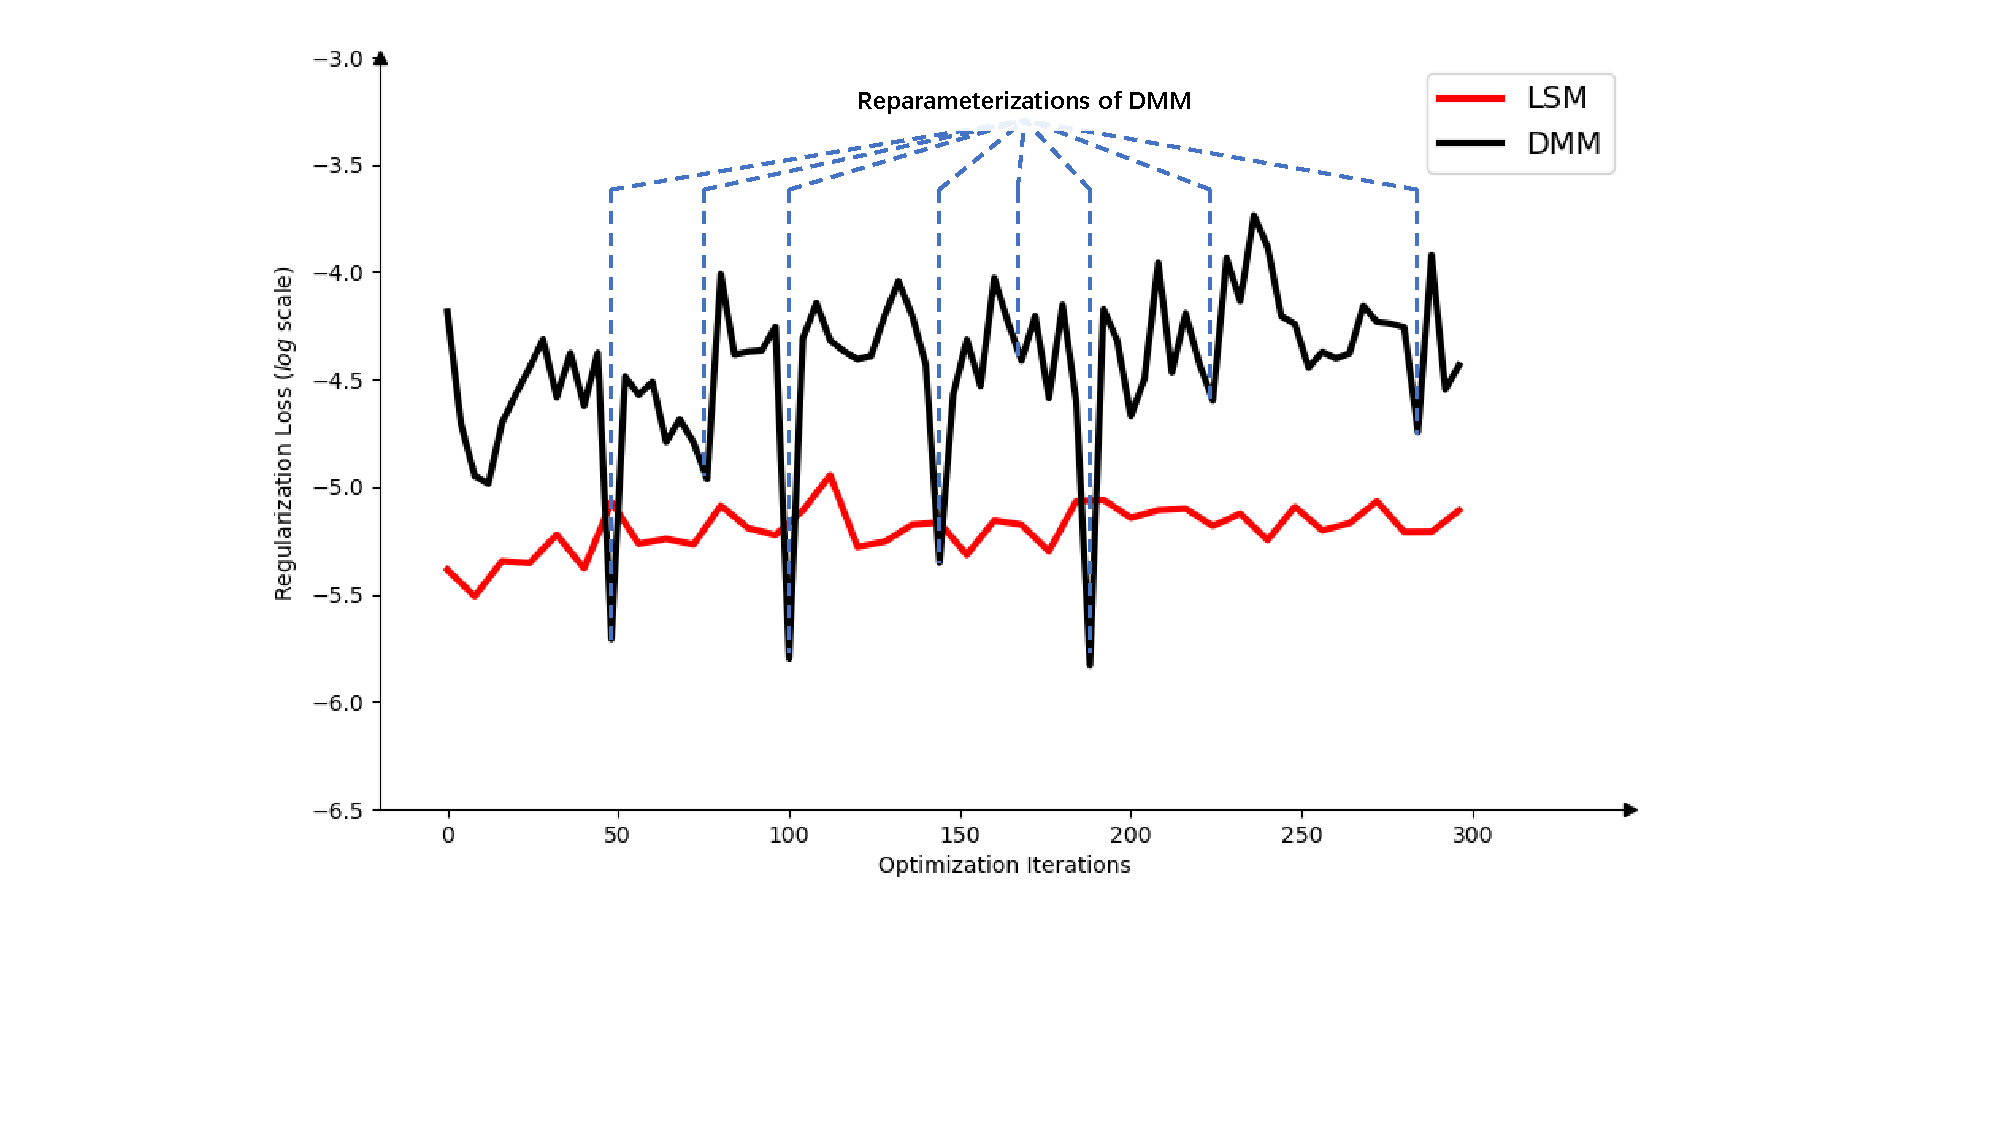
\includegraphics[width=0.9\linewidth]{chapter4/fig/lsm_dmm_avm_loss_compare.pdf}
    \end{center}
    \caption{
        \small The comparison of regularization losses of 'LSM+SU2' and 'DMM+SU2' settings. LSM deforms the computational mesh with better quality and less triggers the reparameterization.
    }
    \label{ch4:fig:reg_loss_compare}
\end{figure}

\begin{figure}[!htb]
    \begin{center}
        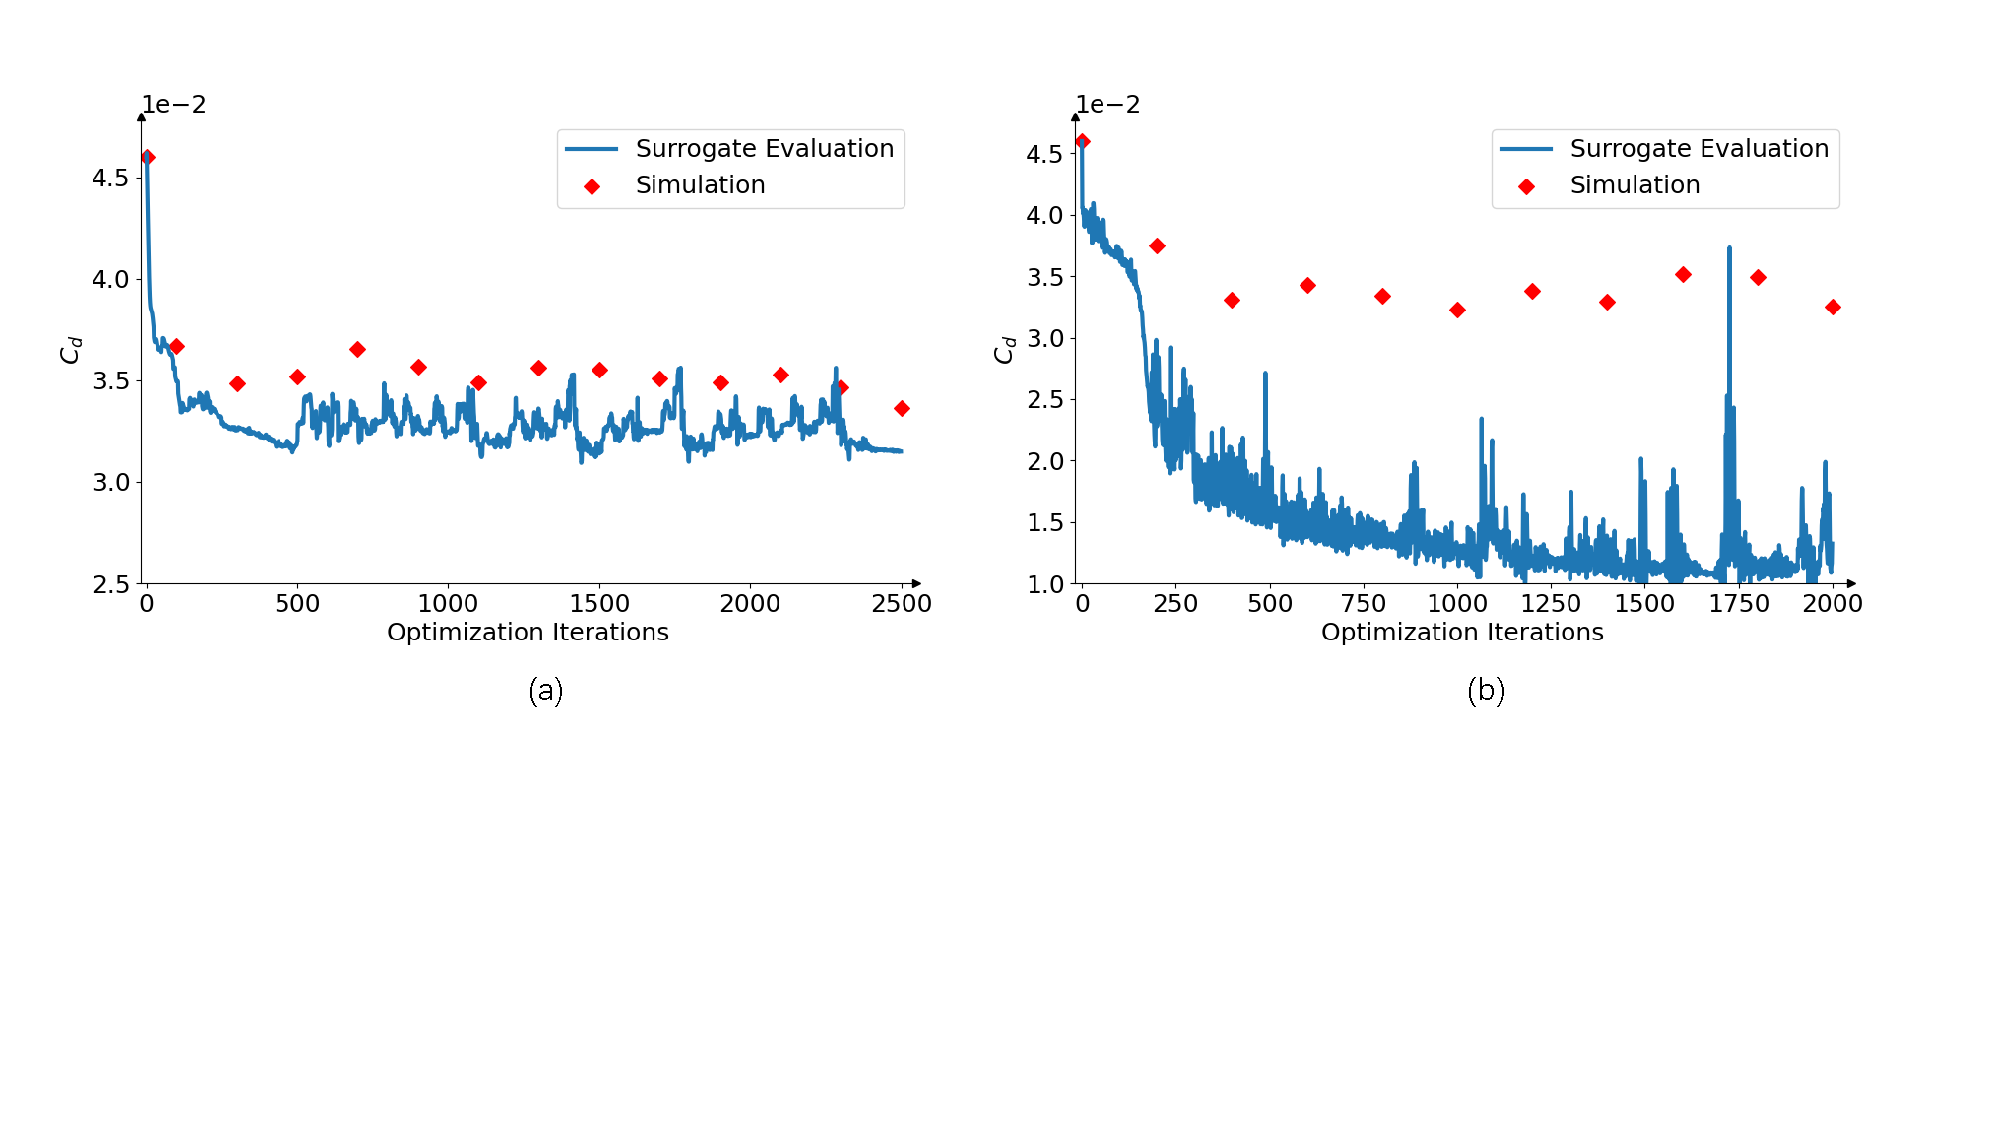
\includegraphics[width=0.9\linewidth]{chapter4/fig/lsm_dmm_gcnn_Cd_history.pdf}
    \end{center}
    \caption{
        \small The gap between GCNN's evaluations and simulation results becomes more significant when the airfoil is more deformed and falls outside the distribution of the training data, when it is combined with (a) LSM and (b) DMM. GCNN shows limited generalization ability when it only relies on a fixed training set.
    }
    \label{ch4:fig:gcnn_gap}
\end{figure}

The optimized NACA-0012 airfoils are shown in Fig.\ref{ch4:fig:final_optim_results}. The drag coefficients are significantly reduced in all four cases, indicating the effectiveness of the proposed parameterization methods with both evaluation models. The quantitative results in Tab.\ref{ch4:tab:result} demonstrate that the proposed automatic parameterization models perform comparably to previous handcrafted and semi-automatic parameterizations. However, the results differ between cases. Specifically, DMM generates larger deformations than LSM, which aligns with our discussion in Sec.\ref{ch4:sec:discussion_lsm_dmm} that the latent space of LSM parameterizes the distribution of the training dataset, while the optimal result obtained by \textit{DMM + SU2} does not follow the distribution of NACA profiles and the UIUC airfoil dataset. LSM provides simpler geometric constraints and better computational mesh deformation. As illustrated in Fig.\ref{ch4:fig:reg_loss_compare}, \textit{LSM + SU2} has a lower regularization loss value than \textit{DMM + SU2}, and no reparameterization is triggered during optimization.

In terms of evaluation models, SU2 consistently outperforms the GCNN model due to the limited generalization ability of GCNN. This limitation arises because the training set of GCNN includes fluid data only from existing airfoils. In this case, the optimized airfoils become out-of-distribution data, resulting in a large gap between the evaluation result and the real aerodynamic performance, as shown in Fig.\ref{ch4:fig:gcnn_gap}. This phenomenon makes it unsuitable for guiding the optimization process in the latter stage. However, SU2 takes considerably more computational time than GCNN. When both perform 100 iterations, using the GCNN model costs $9s$, while SU2 costs $2253s$ on the coarse template mesh \textit{TM-A}.
